\begin{figure}[ht]
	\begin{tabularx}{.8\linewidth}{Y Y}
		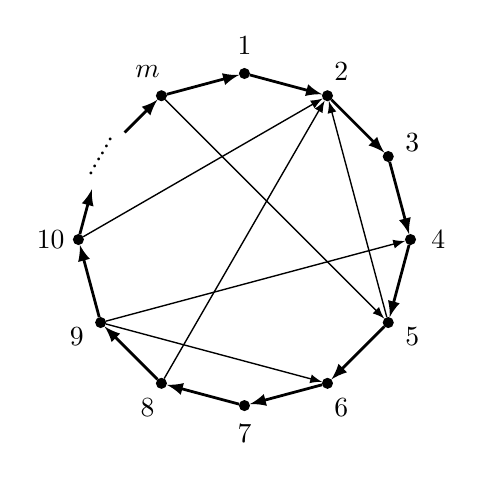
\begin{tikzpicture}
			\foreach \angle [count = \xi] in {90, 60, ..., -180}
				{
					\node[circle, fill, minimum size=.4em, inner sep=0pt, outer sep=0pt] (node\xi) at (\angle:6em) {};
					\node (nodetext\xi) at (\angle:7em) {\xi};
				}
			\node[circle, fill, minimum size=.4em, inner sep=0pt, outer sep=0pt] (node12) at (120:6em) {};
			\node (nodetext12) at (120:7em) {$m$};
			\node[rotate = 60] (node11) at (150:6em) {......};
			\draw[-latex,line width = .1em] (node12) -- (node1);
			\foreach \xi in {2, 3, ..., 12}
				{
					\pgfmathtruncatemacro\xii{\xi - 1};
					\draw[-latex,line width = .1em] (node\xii) -- (node\xi);
				}
			\foreach \x/\y in {12/5, 10/2, 8/2, 5/2, 9/4, 9/6}
				{
					\draw[-latex,line width = .05em] (node\x) -- (node\y);
				}
		\end{tikzpicture}
		 &
		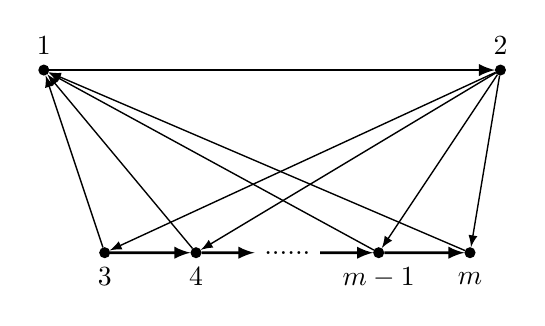
\begin{tikzpicture}[scale=1.1]
			\node[circle, fill, minimum size=.4em, inner sep=0pt, outer sep=0pt, label=above:1] (node1) {};
			\node[circle, fill, minimum size=.4em, inner sep=0pt, outer sep=0pt, label=above:2] at ([xshift = 15em]node1)(node2) {};
			\draw[-latex,line width = .1em] (node1) -- (node2);
			\node[circle, fill, minimum size=.4em, inner sep=0pt, outer sep=0pt, label=below:{3}]  at ([xshift = 2em, yshift = -6em]node1) (node31) {};
			\node[circle, fill, minimum size=.4em, inner sep=0pt, outer sep=0pt, label=below:{4}]  at ([xshift = 5em, yshift = -6em]node1) (node32) {};
			\node at ([xshift = 8em, yshift = -6em]node1) (node33) {......};
			\node[circle, fill, minimum size=.4em, inner sep=0pt, outer sep=0pt, label=below:{$m - 1$}]  at ([xshift = 11em, yshift = -6em]node1) (node34) {};
			\node[circle, fill, minimum size=.4em, inner sep=0pt, outer sep=0pt, label={[label distance = .18em]below:$m$}]  at ([xshift = 14em, yshift = -6em]node1) (node35) {};
			\foreach \i in {1, 2, 4, 5}
				{
					\draw[-latex,line width = .05em] (node2) -- (node3\i);
					\draw[-latex,line width = .05em] (node3\i) -- (node1);
				}

			\foreach \i [count = \xi] in {2, ..., 5}
				{
					\draw[-latex,line width = .1em] (node3\xi) -- (node3\i);
				}
		\end{tikzpicture}
		\\
		(a) \textsf{Aequitas}
		 &
		(b) \textsf{pompe}
		\\
	\end{tabularx}
    \addtocounter{table}{-1}
	\medskip
	
	\caption{Illustration of dependency graphs.}
	\label{fig:bad-bandwidth-illustration}
\end{figure}